\documentclass[11pt]{article}
%Gummi|065|=)
\title{}
\author{}
\date{}

\usepackage{graphicx}
\usepackage{caption}
\usepackage{subcaption}
\usepackage{gensymb}

\begin{document}

\newpage
\begin{figure}

	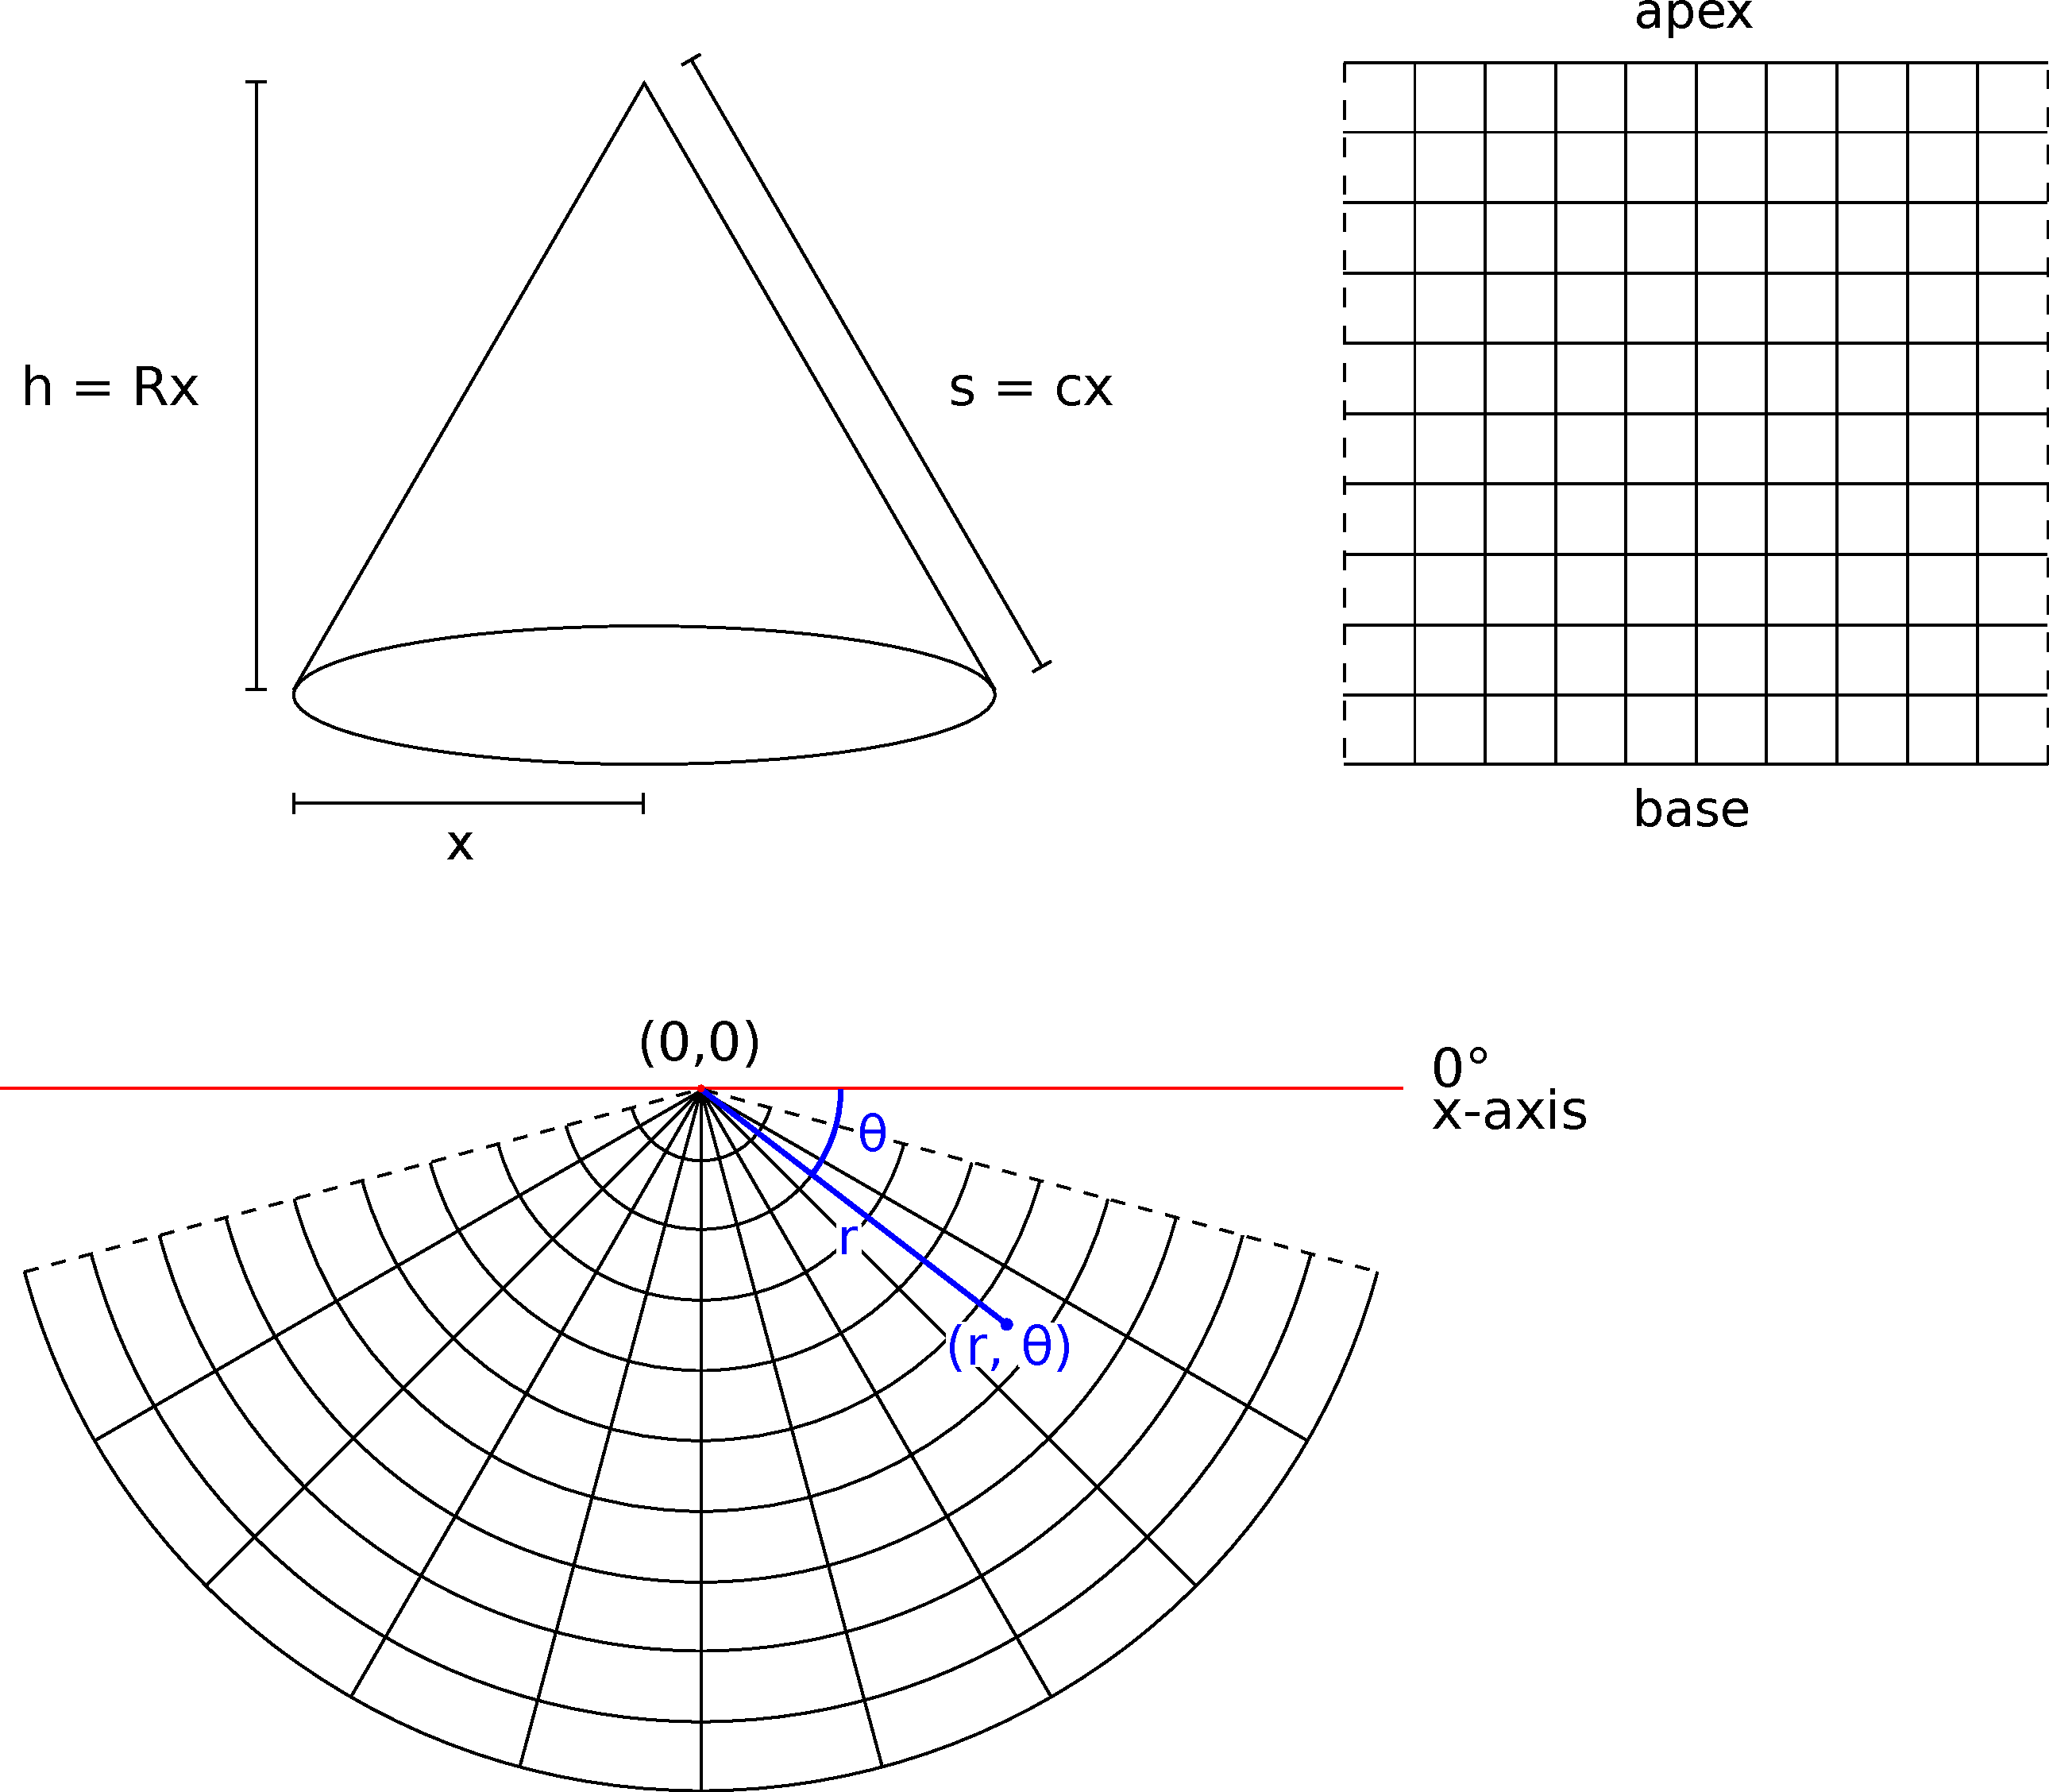
\includegraphics[width=1\linewidth]{ConeGrid_r_theta.pdf}

	\caption{The model mountain is a cone. Unfurled, a cone's surface is a circle sector. The polar coordinates, $r$ and $\theta$, describe position on the mountain. The circle centre (mountain tip or cone apex) is the origin, (0, 0). In silico, I represent the cone's surface as a square array (grid of cells). Rows in the array are altitudinal bands, and columns, positions along a band. Row indices correspond to radial positions, and column indices, to angular positions. The array's top edge is the cone's apex (mountain tip). The cone has three parameters: base radius ($x$), height ($h$), and slant height ($s$).}

\end{figure}


\newpage
\begin{figure}
\vspace*{-4cm}

	\begin{subfigure}{\textwidth}
		\centering
		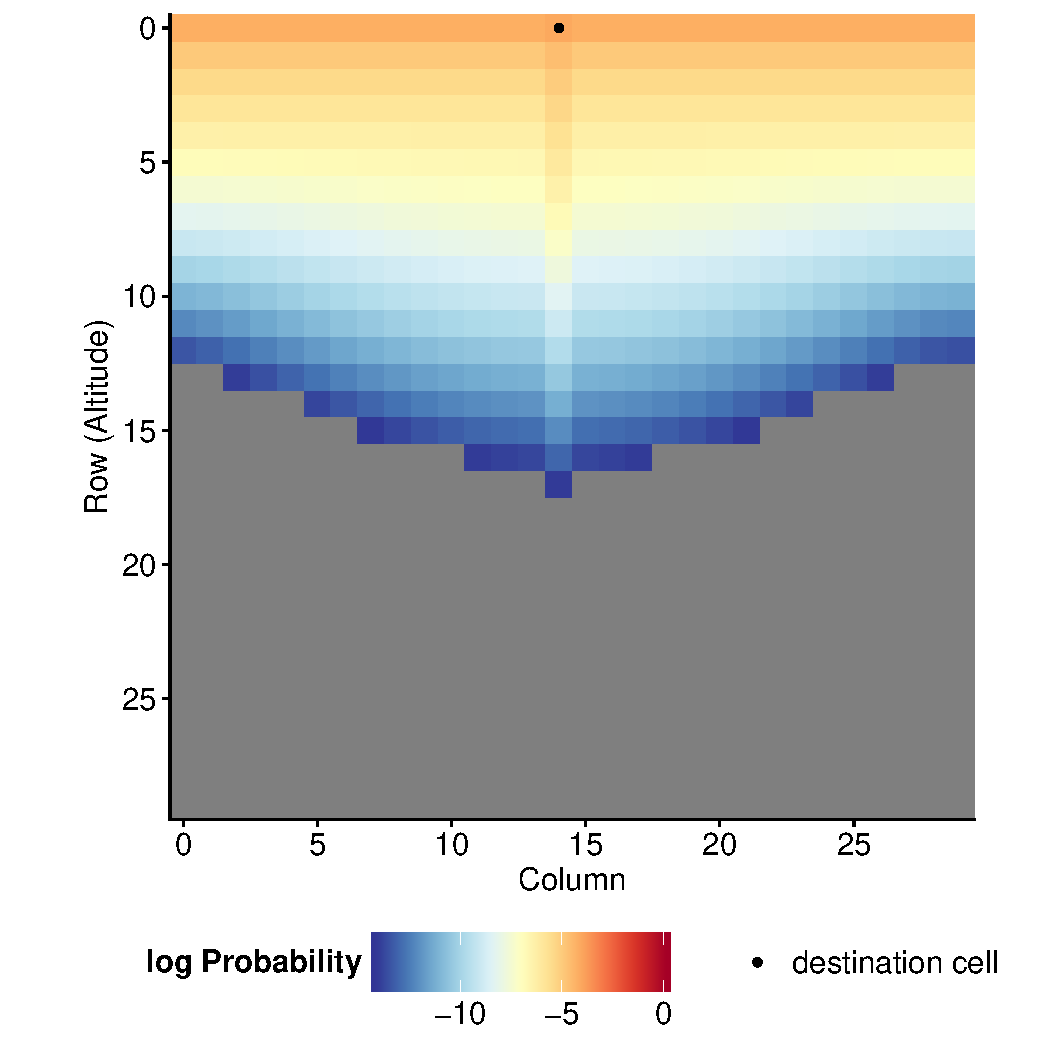
\includegraphics[width=0.6\linewidth]{../Results/DispMaps/AreaNoTemp100Top.pdf}
		\caption{}
	\end{subfigure}%

	\begin{subfigure}{\textwidth}
		\centering
		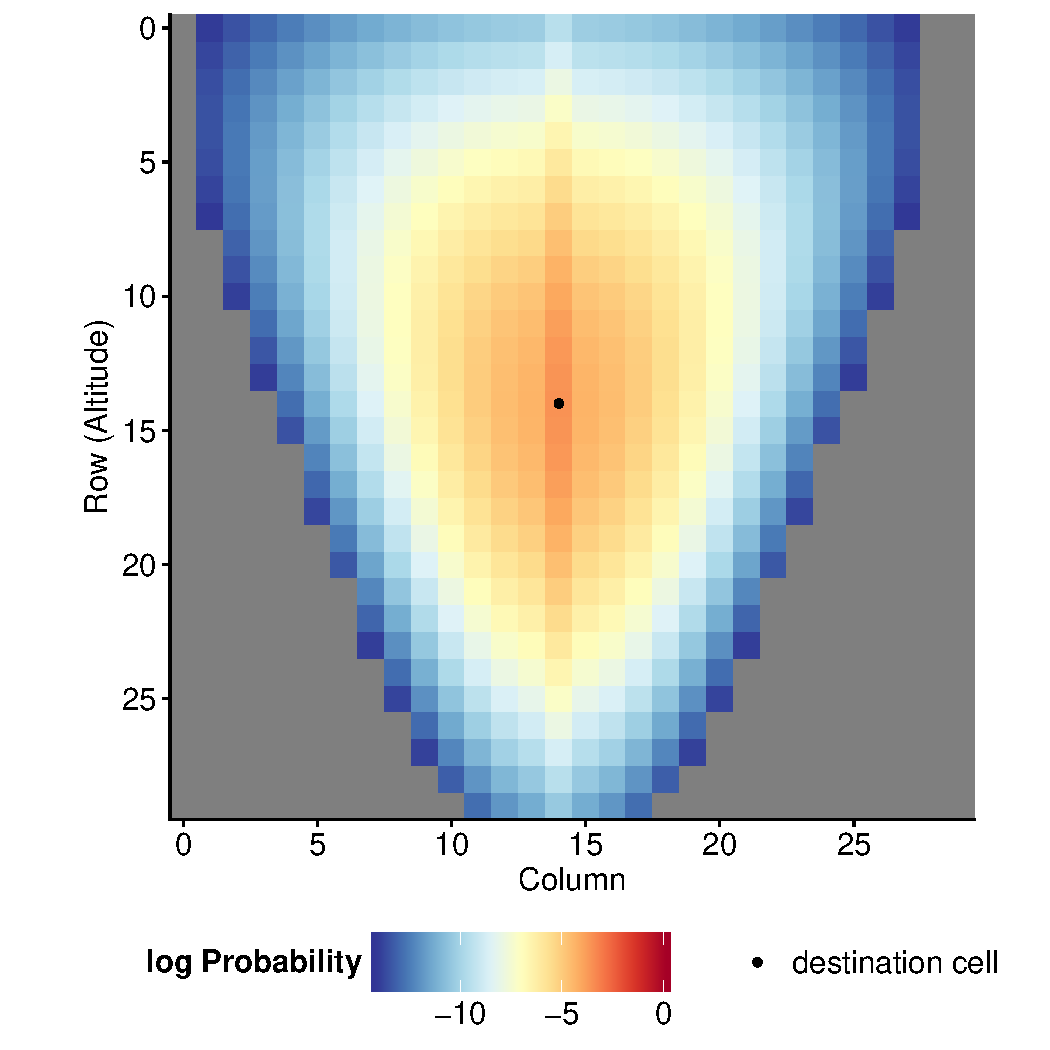
\includegraphics[width=0.6\linewidth]{../Results/DispMaps/AreaNoTemp100.pdf}
		\caption{}
	\end{subfigure}

	\begin{subfigure}{\textwidth}
		\centering
		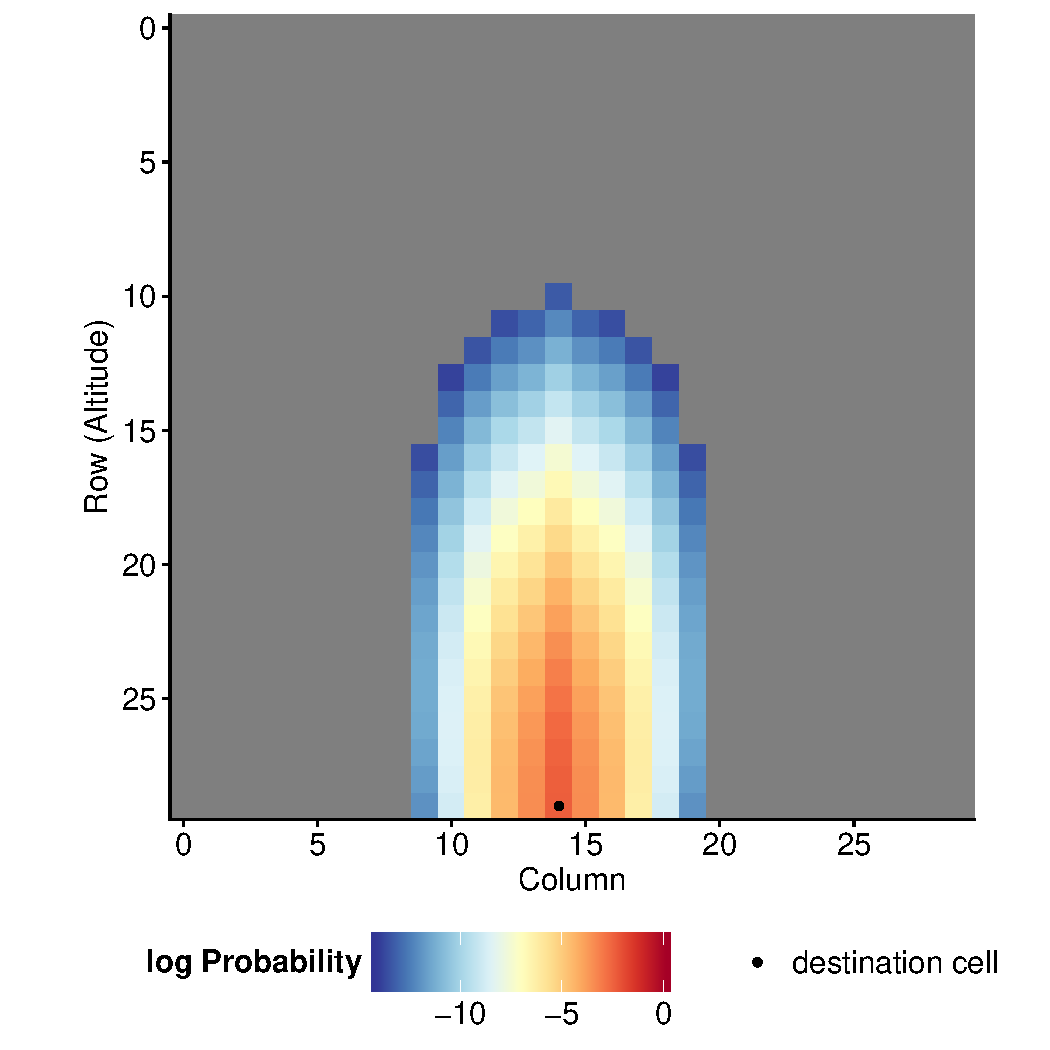
\includegraphics[width=0.6\linewidth]{../Results/DispMaps/AreaNoTemp100Bottom.pdf}
		\caption{}
	\end{subfigure}

	\caption{The effect of area without temperature. Log probability of dispersing to a destination at the top, middle, and bottom of the mountain. Grey squares represent probability $\leq 1 \times 10^{-6}$. (Temperature fixed to 15 \degree C; body mass 100 g.) }

\end{figure}


\newpage
\begin{figure}
\vspace*{-6cm}
\centering

	\begin{subfigure}{\textwidth}
		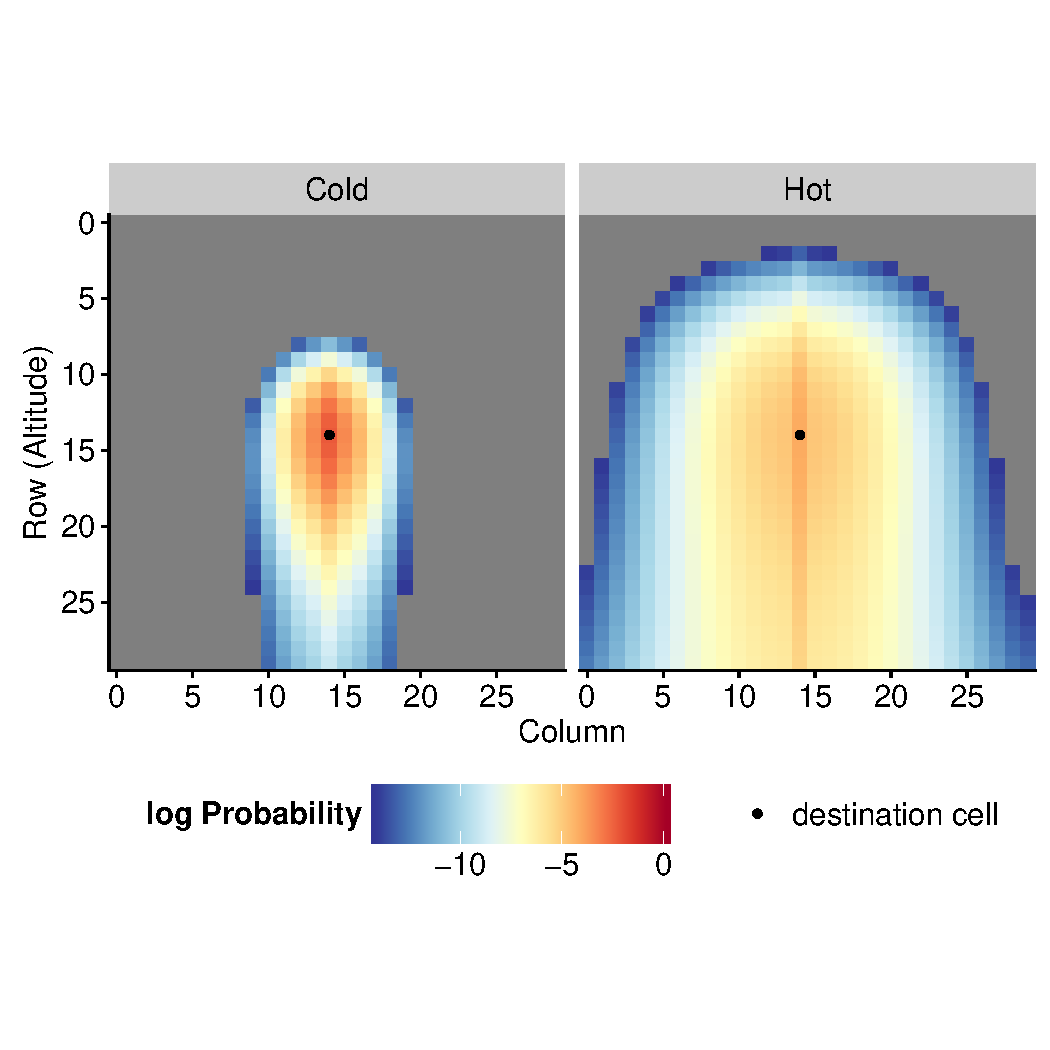
\includegraphics[width=1\linewidth]{../Results/DispMaps/AreaTemp_ColdHot.pdf}
		\caption{The effect of adding a temperature gradient. Comparison between cold (temperate, 0-15 \degree C) and hot (tropical, 10-25 \degree C) mountains. (Body mass 100 g; area effect present).}
	\end{subfigure}%
	
	\begin{subfigure}{\textwidth}
		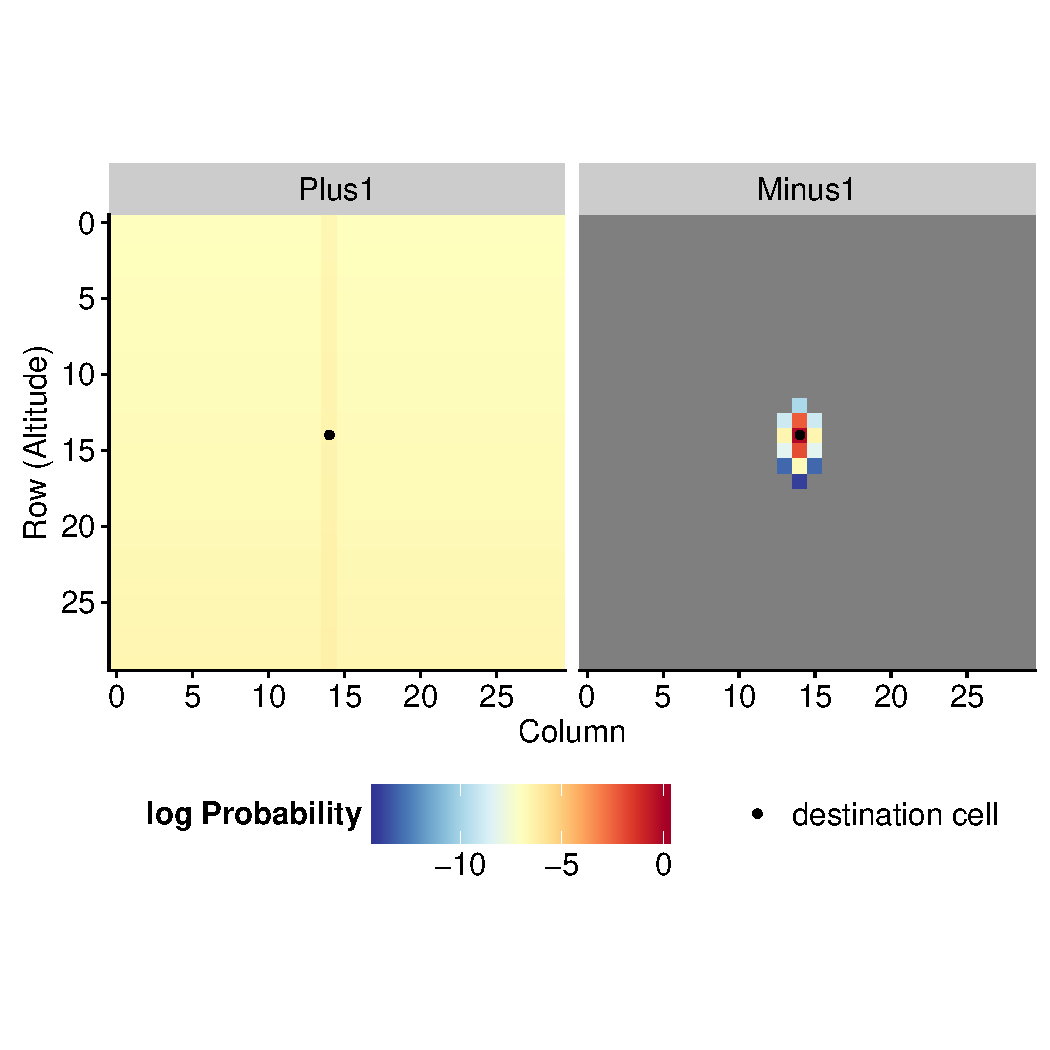
\includegraphics[width=1\linewidth]{../Results/DispMaps/AreaTemp_B0.pdf}
		\caption{Making mountains out of molehills. Increasing/reducing the normalisation constant for dispersal by an order of magnitude. (Area and temperature effects present).}
	\end{subfigure}%

	\caption{}

\end{figure}


\newpage
\begin{figure}

	\begin{subfigure}{\textwidth}
		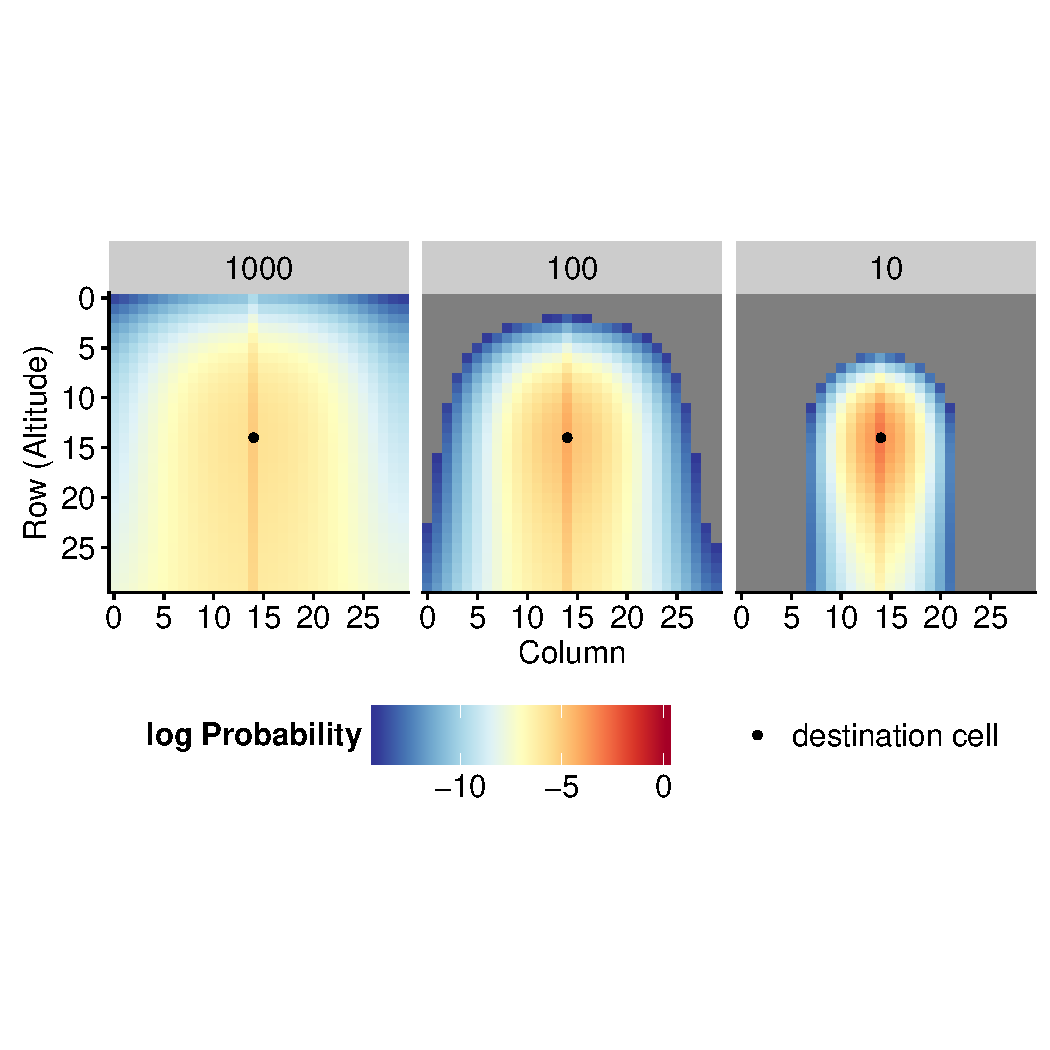
\includegraphics[trim=3cm 0 0 0cm]{../Results/DispMaps/AreaTemp.pdf}
		\caption{}
	\end{subfigure}%

	\caption{Comparison of body sizes, across two orders of magnitude. (Area and temperature effects present; 10-25 \degree C).}

\end{figure}


%\newpage
%\begin{figure}

%	\begin{subfigure}{\textwidth}
%		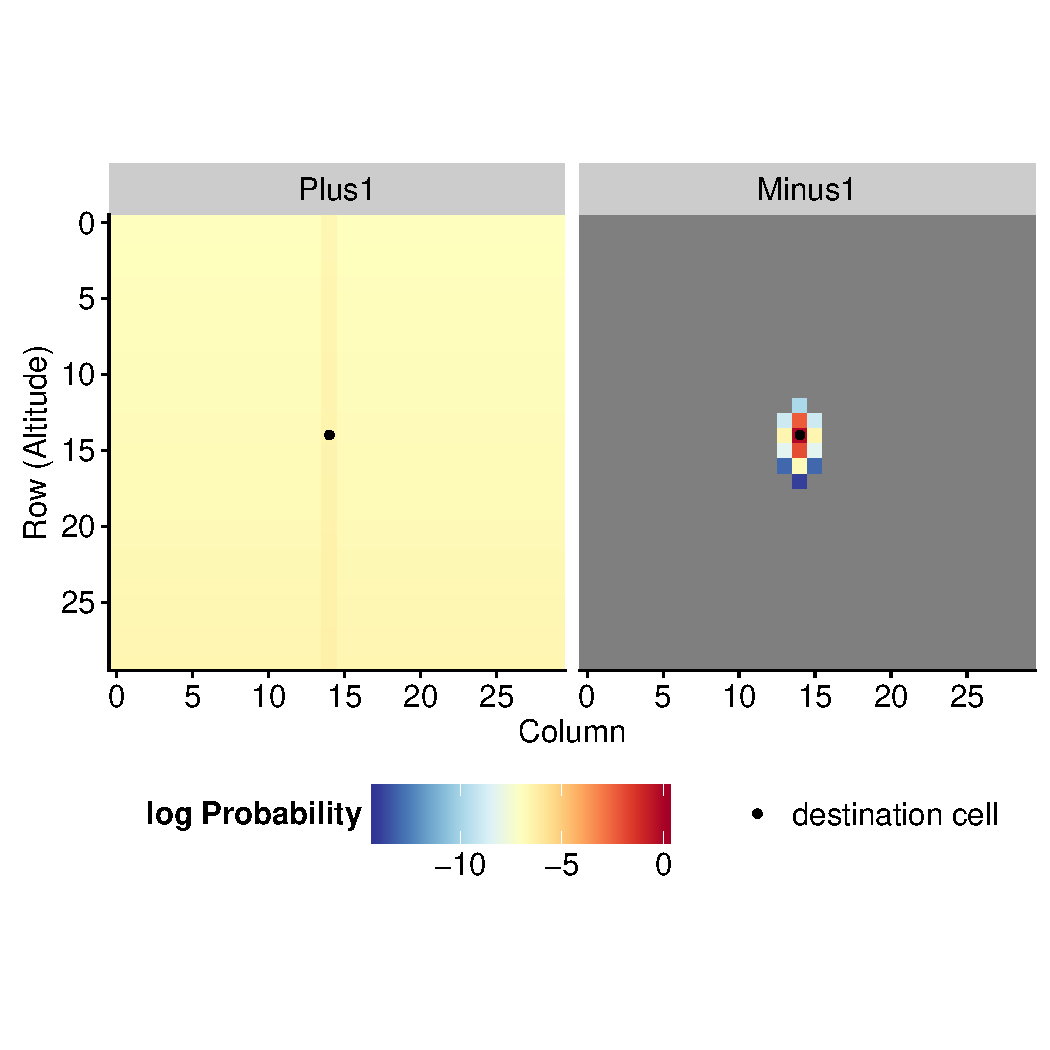
\includegraphics[trim=3cm 0 0 0cm]{../Results/DispMaps/AreaTemp_B0.pdf}
%		\caption{}
%	\end{subfigure}%

%	\caption{}

%\end{figure}


\newpage
\begin{figure}
\vspace*{-7cm}

	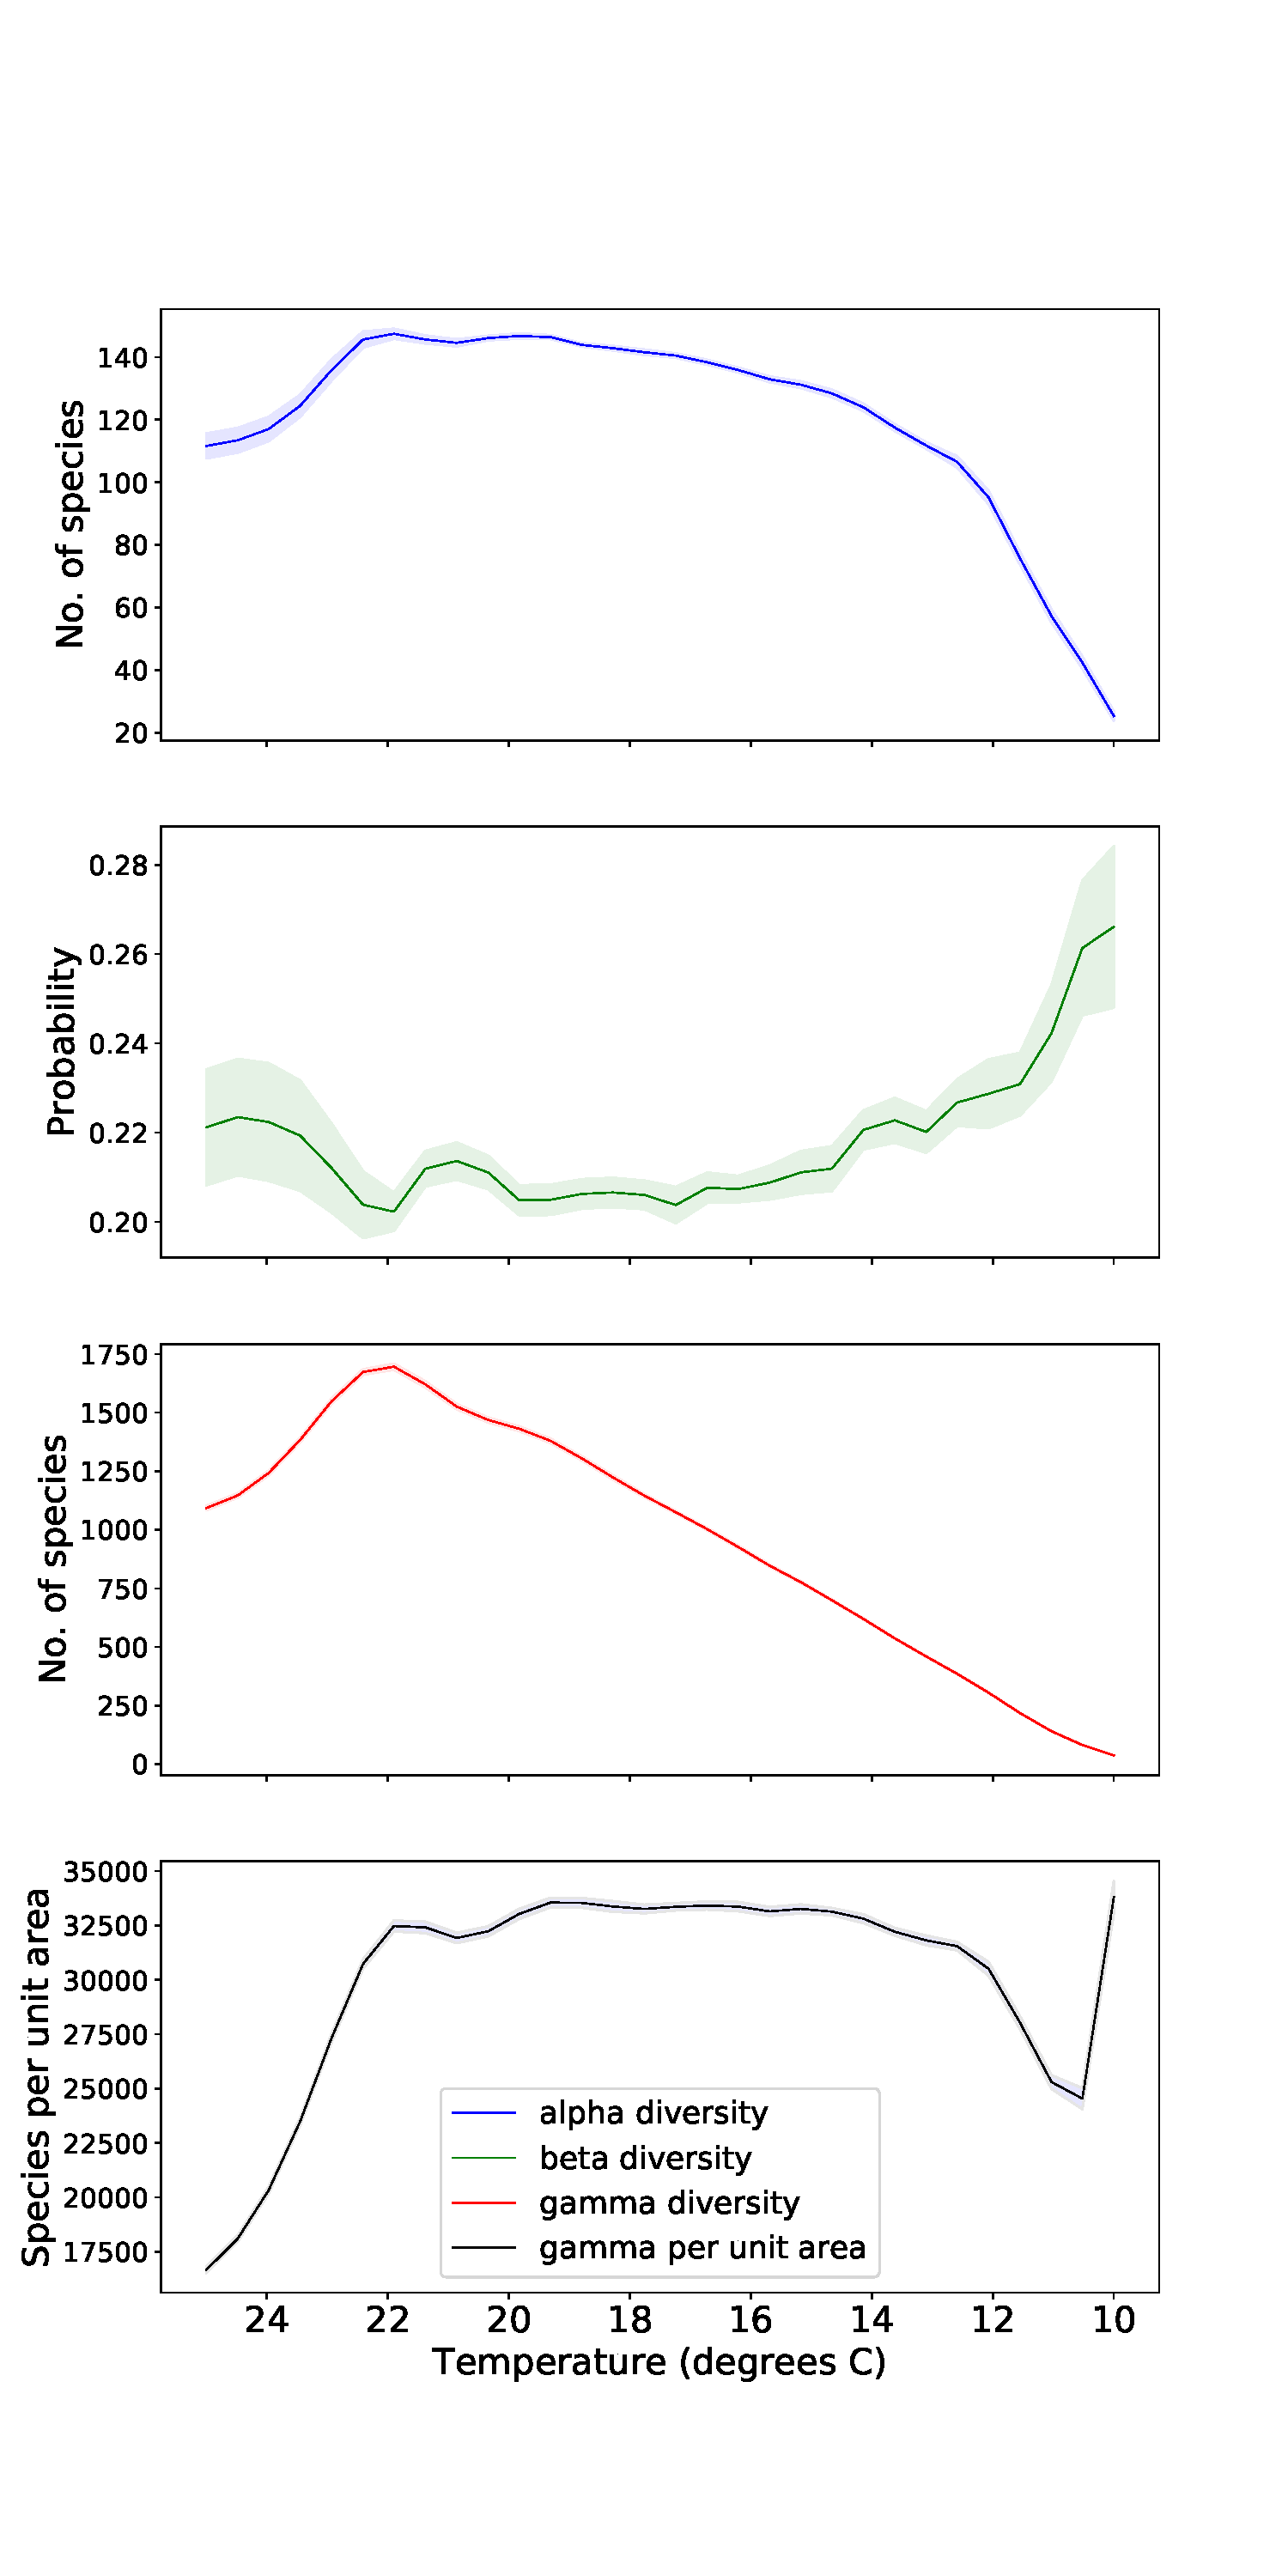
\includegraphics[width=1\linewidth]{../Results/DiversityPlots/100.pdf}
	\caption{Altitudinal gradients of alpha, beta, and gamma species diversity. Temperature increases with decreasing altitude. Alpha diversity is the mean number of species in a fixed area (per band). Beta diversity is the probability that individuals from opposite sides of the mountain are the same species. Gamma diversity is total number of species; the black line is total number divided by band area.\\\\ T.}

\end{figure}


\newpage
\begin{figure}
\vspace*{-7cm}

	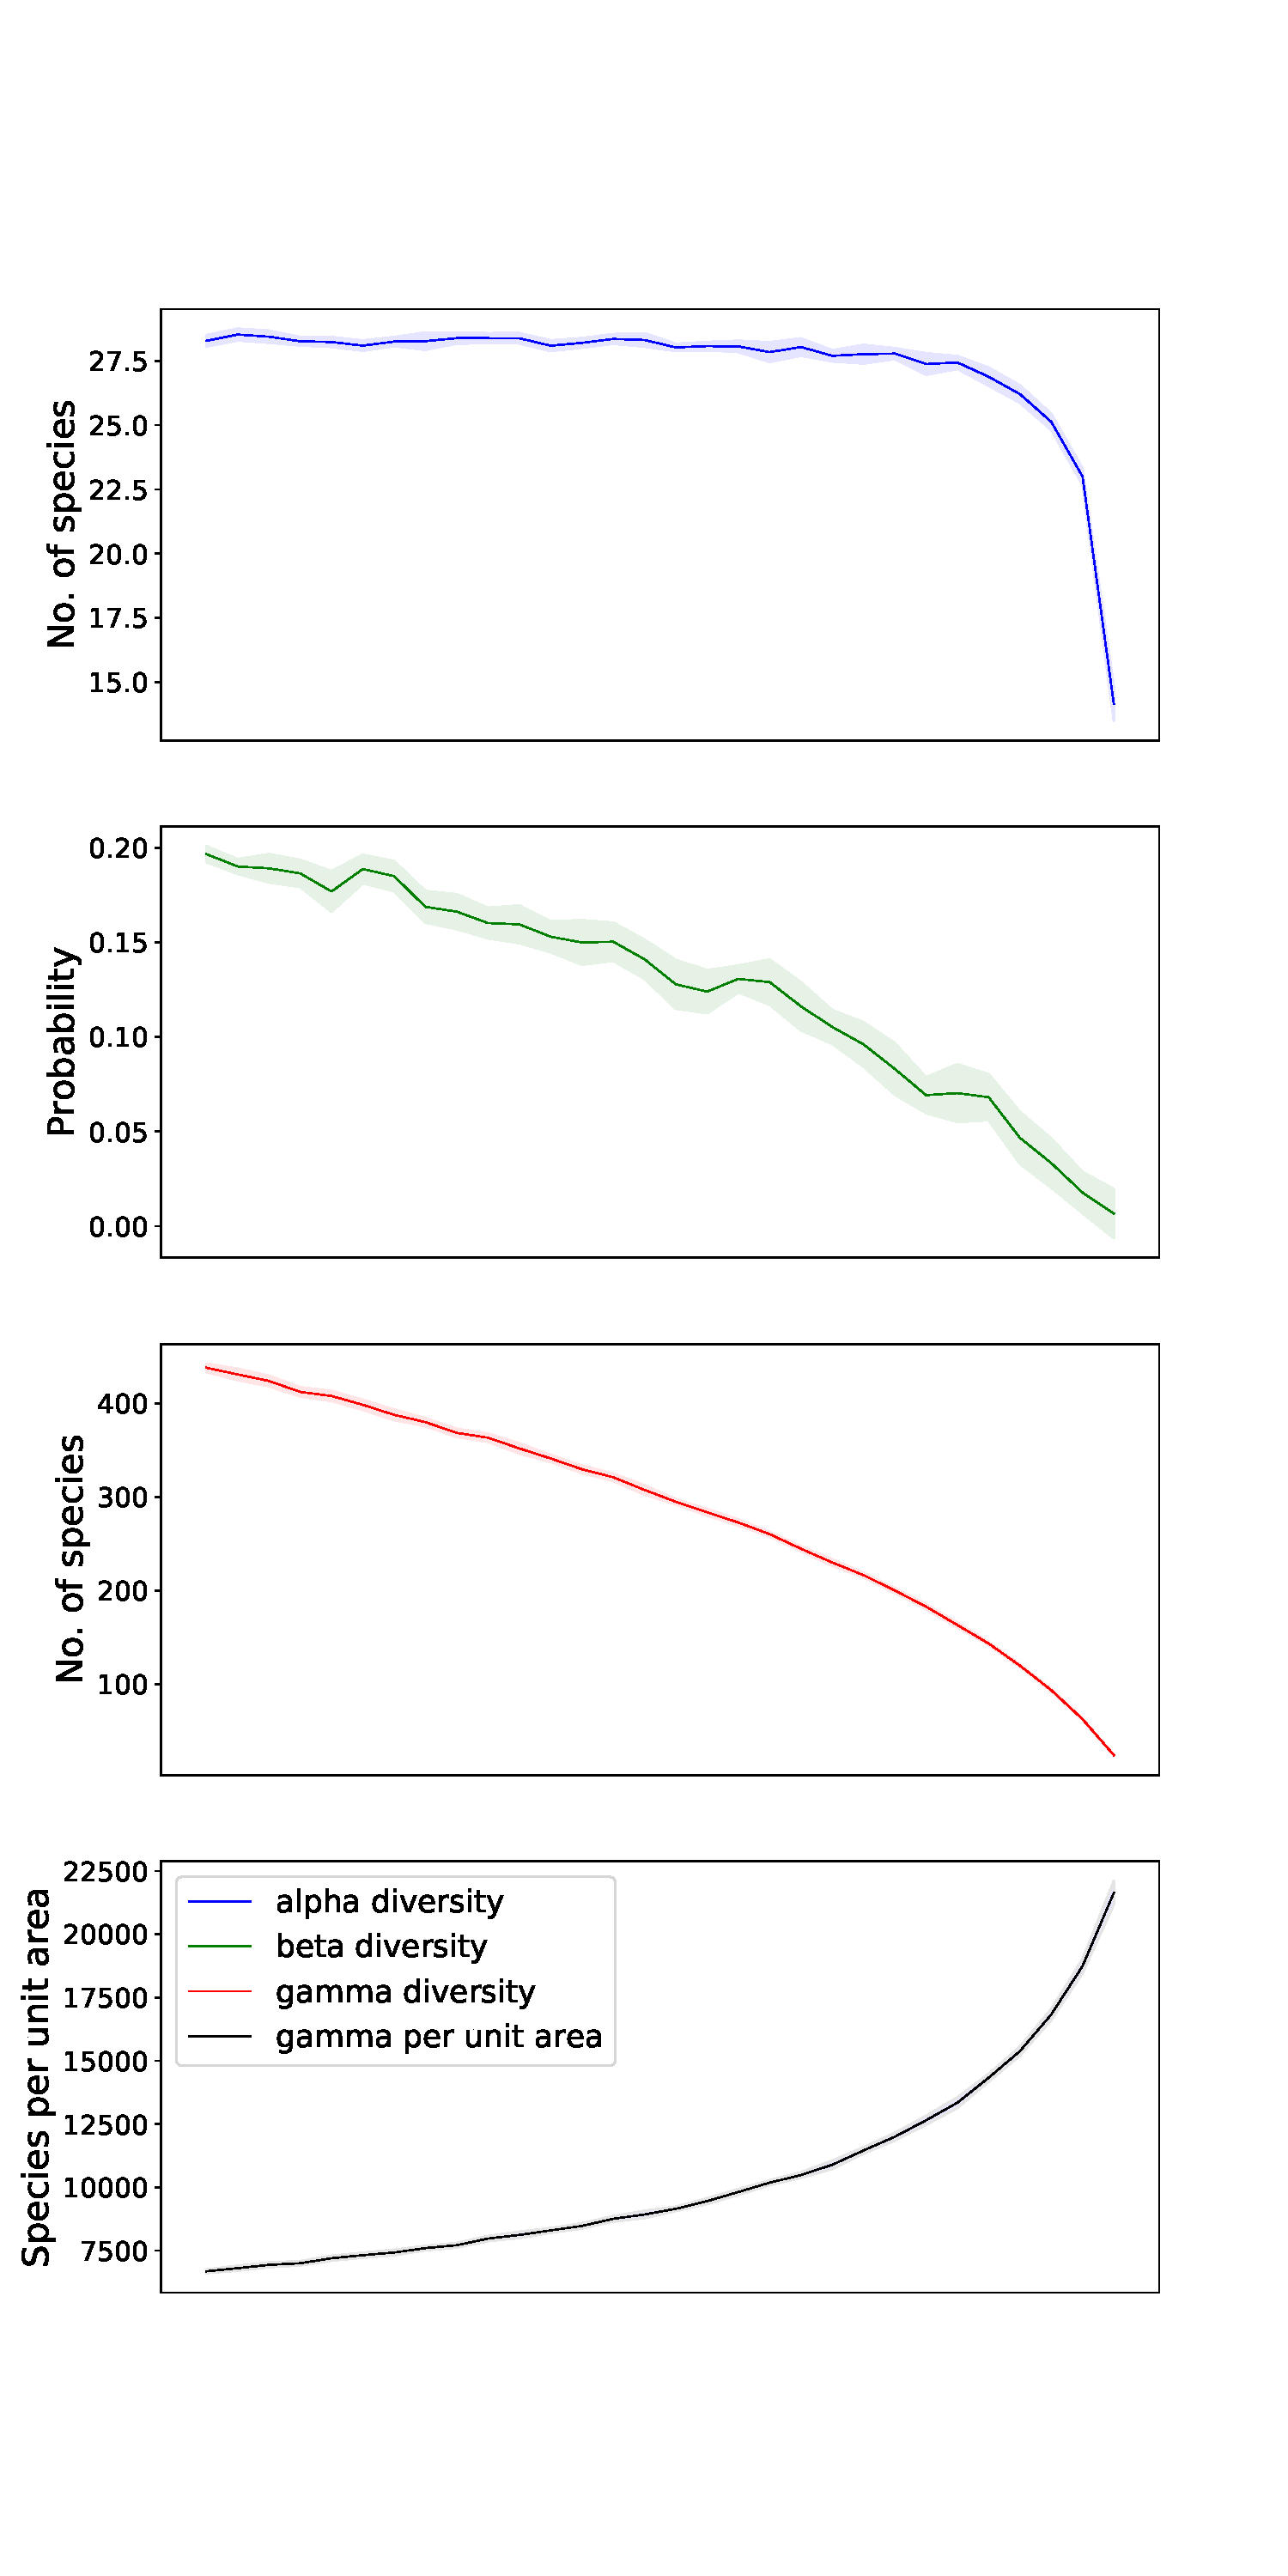
\includegraphics[width=1\linewidth]{../Results/DiversityPlots/AreaNoTemp.pdf}
	\caption{The effect of area without temperature. (Temperature fixed to 15 \degree C; body mass 100 g.)}

\end{figure}


\newpage
\begin{figure}
\vspace*{-7cm}

	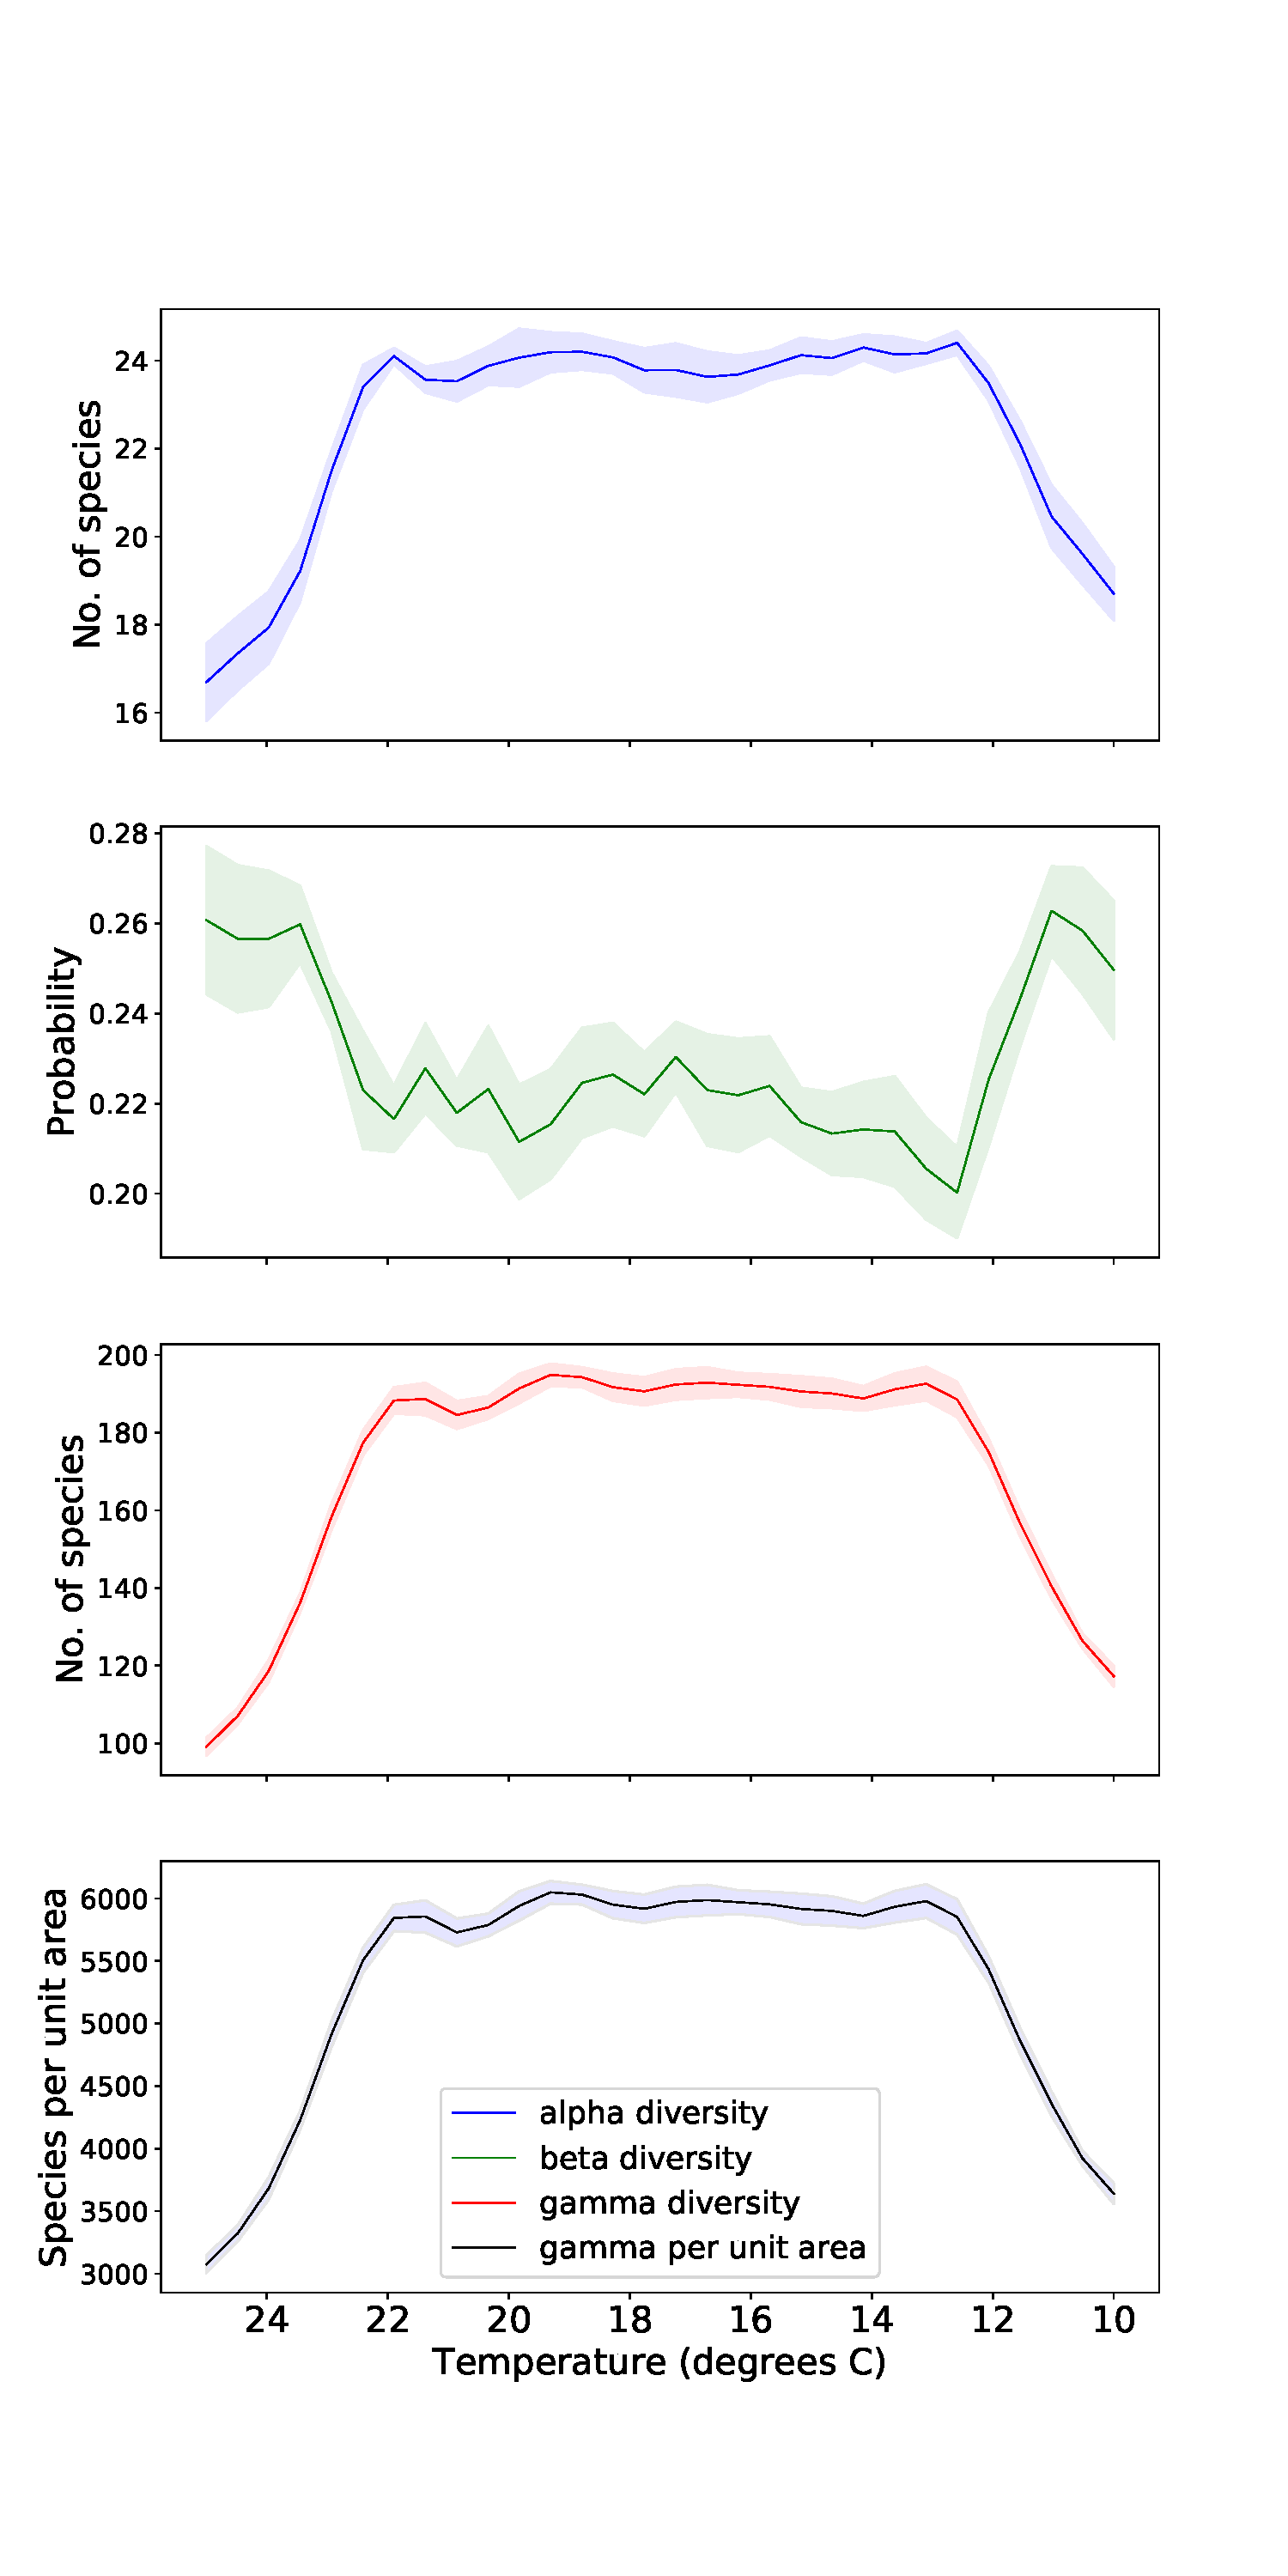
\includegraphics[width=1\linewidth]{../Results/DiversityPlots/TempNoArea.pdf}
	\caption{The effect of temperature - fixed area (system is a cylinder, not cone. Notice alpha diversity - I think the increase in diversity with temperature is either a strong edge effect (high dispersal at hot end, pushing species to the centre) or a bug - I'll look into this.
}

\end{figure}


\end{document}
